\documentclass[10pt]{article}

\usepackage{fullpage}
\usepackage[utf8]{inputenc}
\usepackage[english]{babel}
\usepackage{amssymb}
\usepackage{amsmath}
\usepackage{amsthm}
\usepackage{graphicx}
\usepackage{pdfpages}
%\usepackage{pgf}
%\usepackage{pgfplots}
%\usepackage{tikz}

\title{Assignment 6: Lorenz Attractor}
\author{Zeke T. Estes}
\date{\today}

\begin{document}
\maketitle

\section{Introduction}
To begin the analysis of understanding what exactly the Lorenz Attractor really is, the concept of what an attractor is must first be examined. An attractor is "a set of states (points in the phase space), invariant under the dynamics, towards which neighboring states in a given basin of attraction asymptotically approach in the course of dynamic evolution." \cite{WolframA}. Understanding this, the Lorenz Attractor covers the same principals. The attractor "arises in a simplified system of equations describing the two-dimensional flow of fluid". \cite{WolframLA} 

\section{History}
The Lorenz attractor was originally discovered and modeled by Edward Lorenz. Lorenz wanted to go to college and get a degree in mathematics, but due to circumstances in the early 20th century, Lorenz became a meteorologist. Lorenz was mostly interested in weather prediction, because at the time the method of forecasting the weather was mostly guess work, or predictions. Lorenz utilized a number of equations to model the weather in a way that would predict weather days apart, but nothing that would predict weather any farther apart from that. In 1961 Lorenz was running a new simulation, but in the middle of the simulation, new initial conditions were input and set to run again. This seemingly non-consequential action unleashed a discovery very important to mathematical theory. This discovery showed that even seemingly non-consequential errors, or small deferments of values of initial conditions could prove to be "catastrophic". In modern day mathematics this phenomenon is called "sensitive dependence on initial conditions". \cite{History}

\section{Modeling}
Modeling the Lorenz attractor requires an understanding of the function itself. This function is represented below:

\begin{eqnarray}
	\frac{dx}{dt} & = & a(y-x) \\
	\frac{dy}{dt} & = & x(b-z)-y \\
	\frac{dz}{dt} & = & xy-cz
\end{eqnarray}

In the following python program, initial values of a = 10, b = 28, and c = $\frac{8}{3}$ where used to model the Lorenz attractor. 

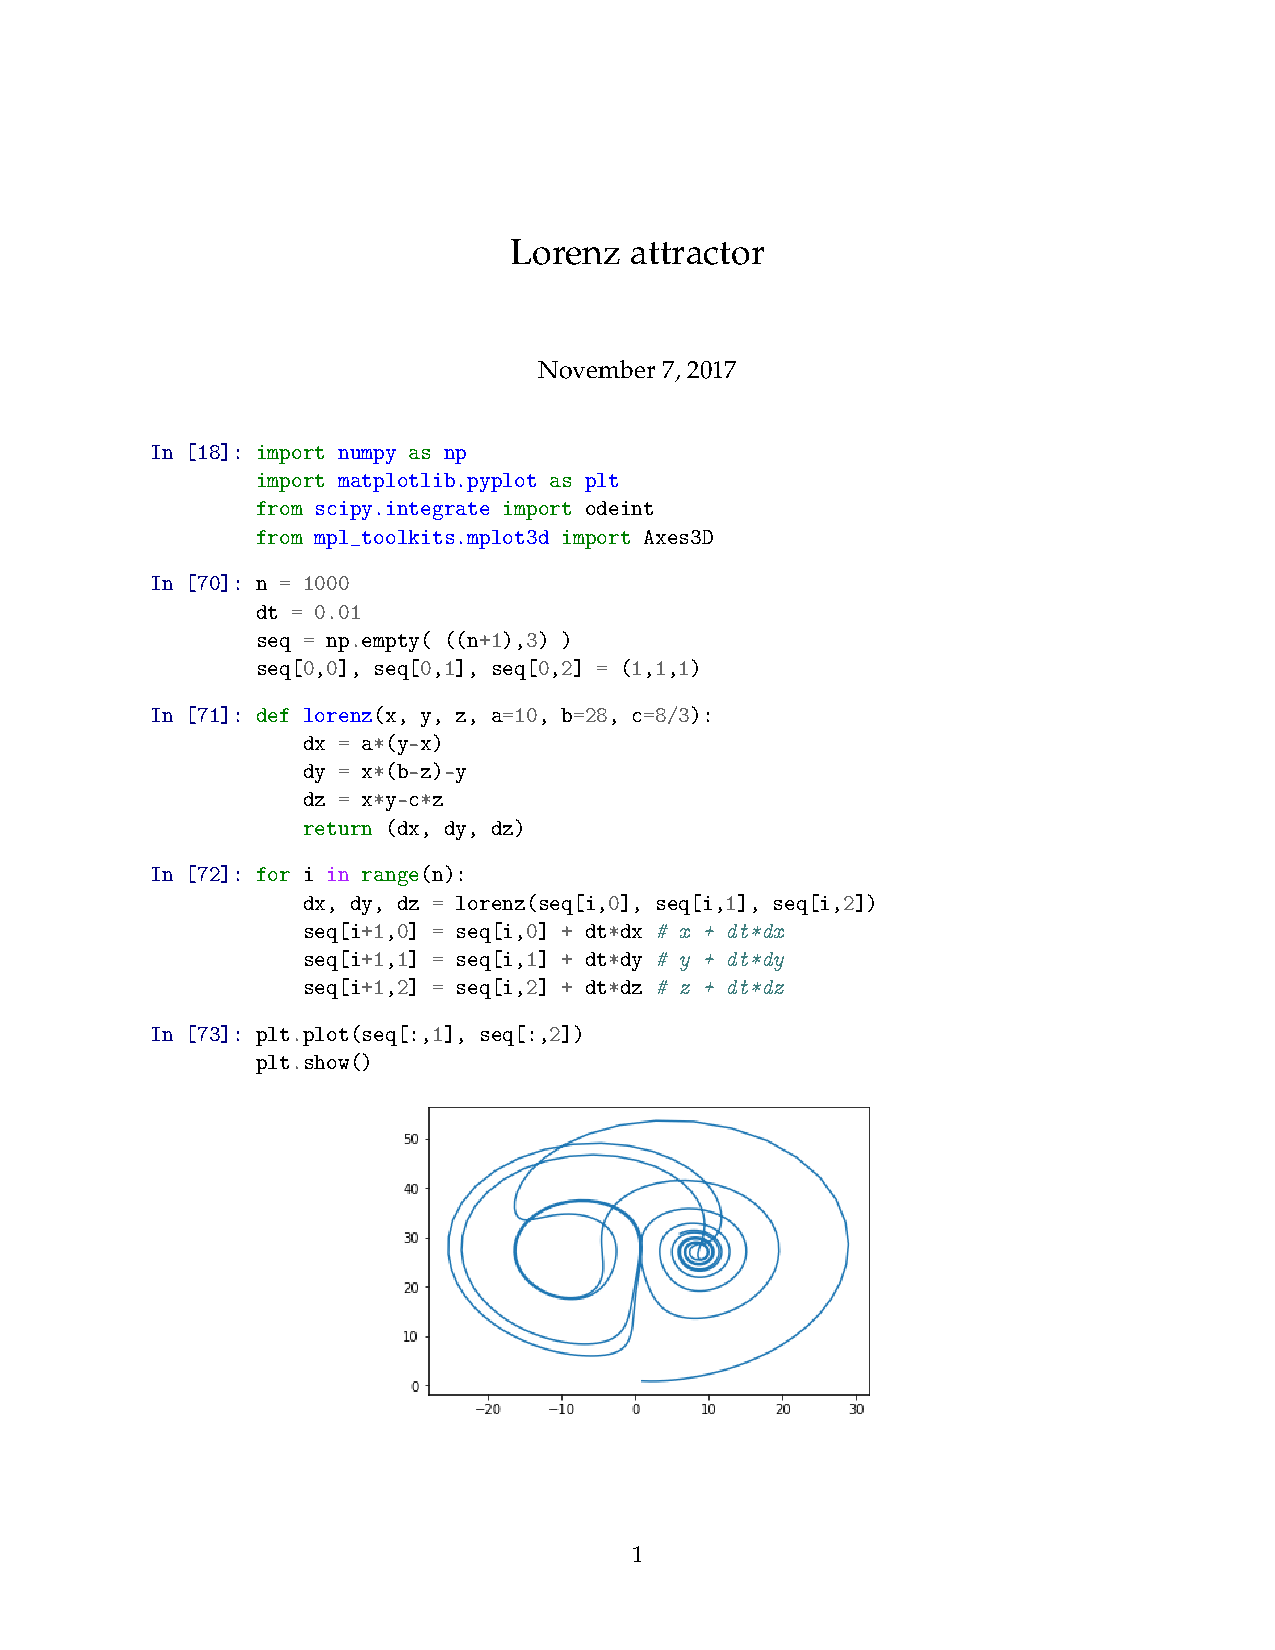
\includepdf[pages=-]{include/program.pdf}

This program quickly diverges and becomes chaotic if the values are changed at all, and if the increments, in this program it is 1000, change than the complexity of the chaos also changes. Another method of plotting this function is also explored using Mathematica. \cite{Mathematica}

\begin{figure}[h]
	\centering
	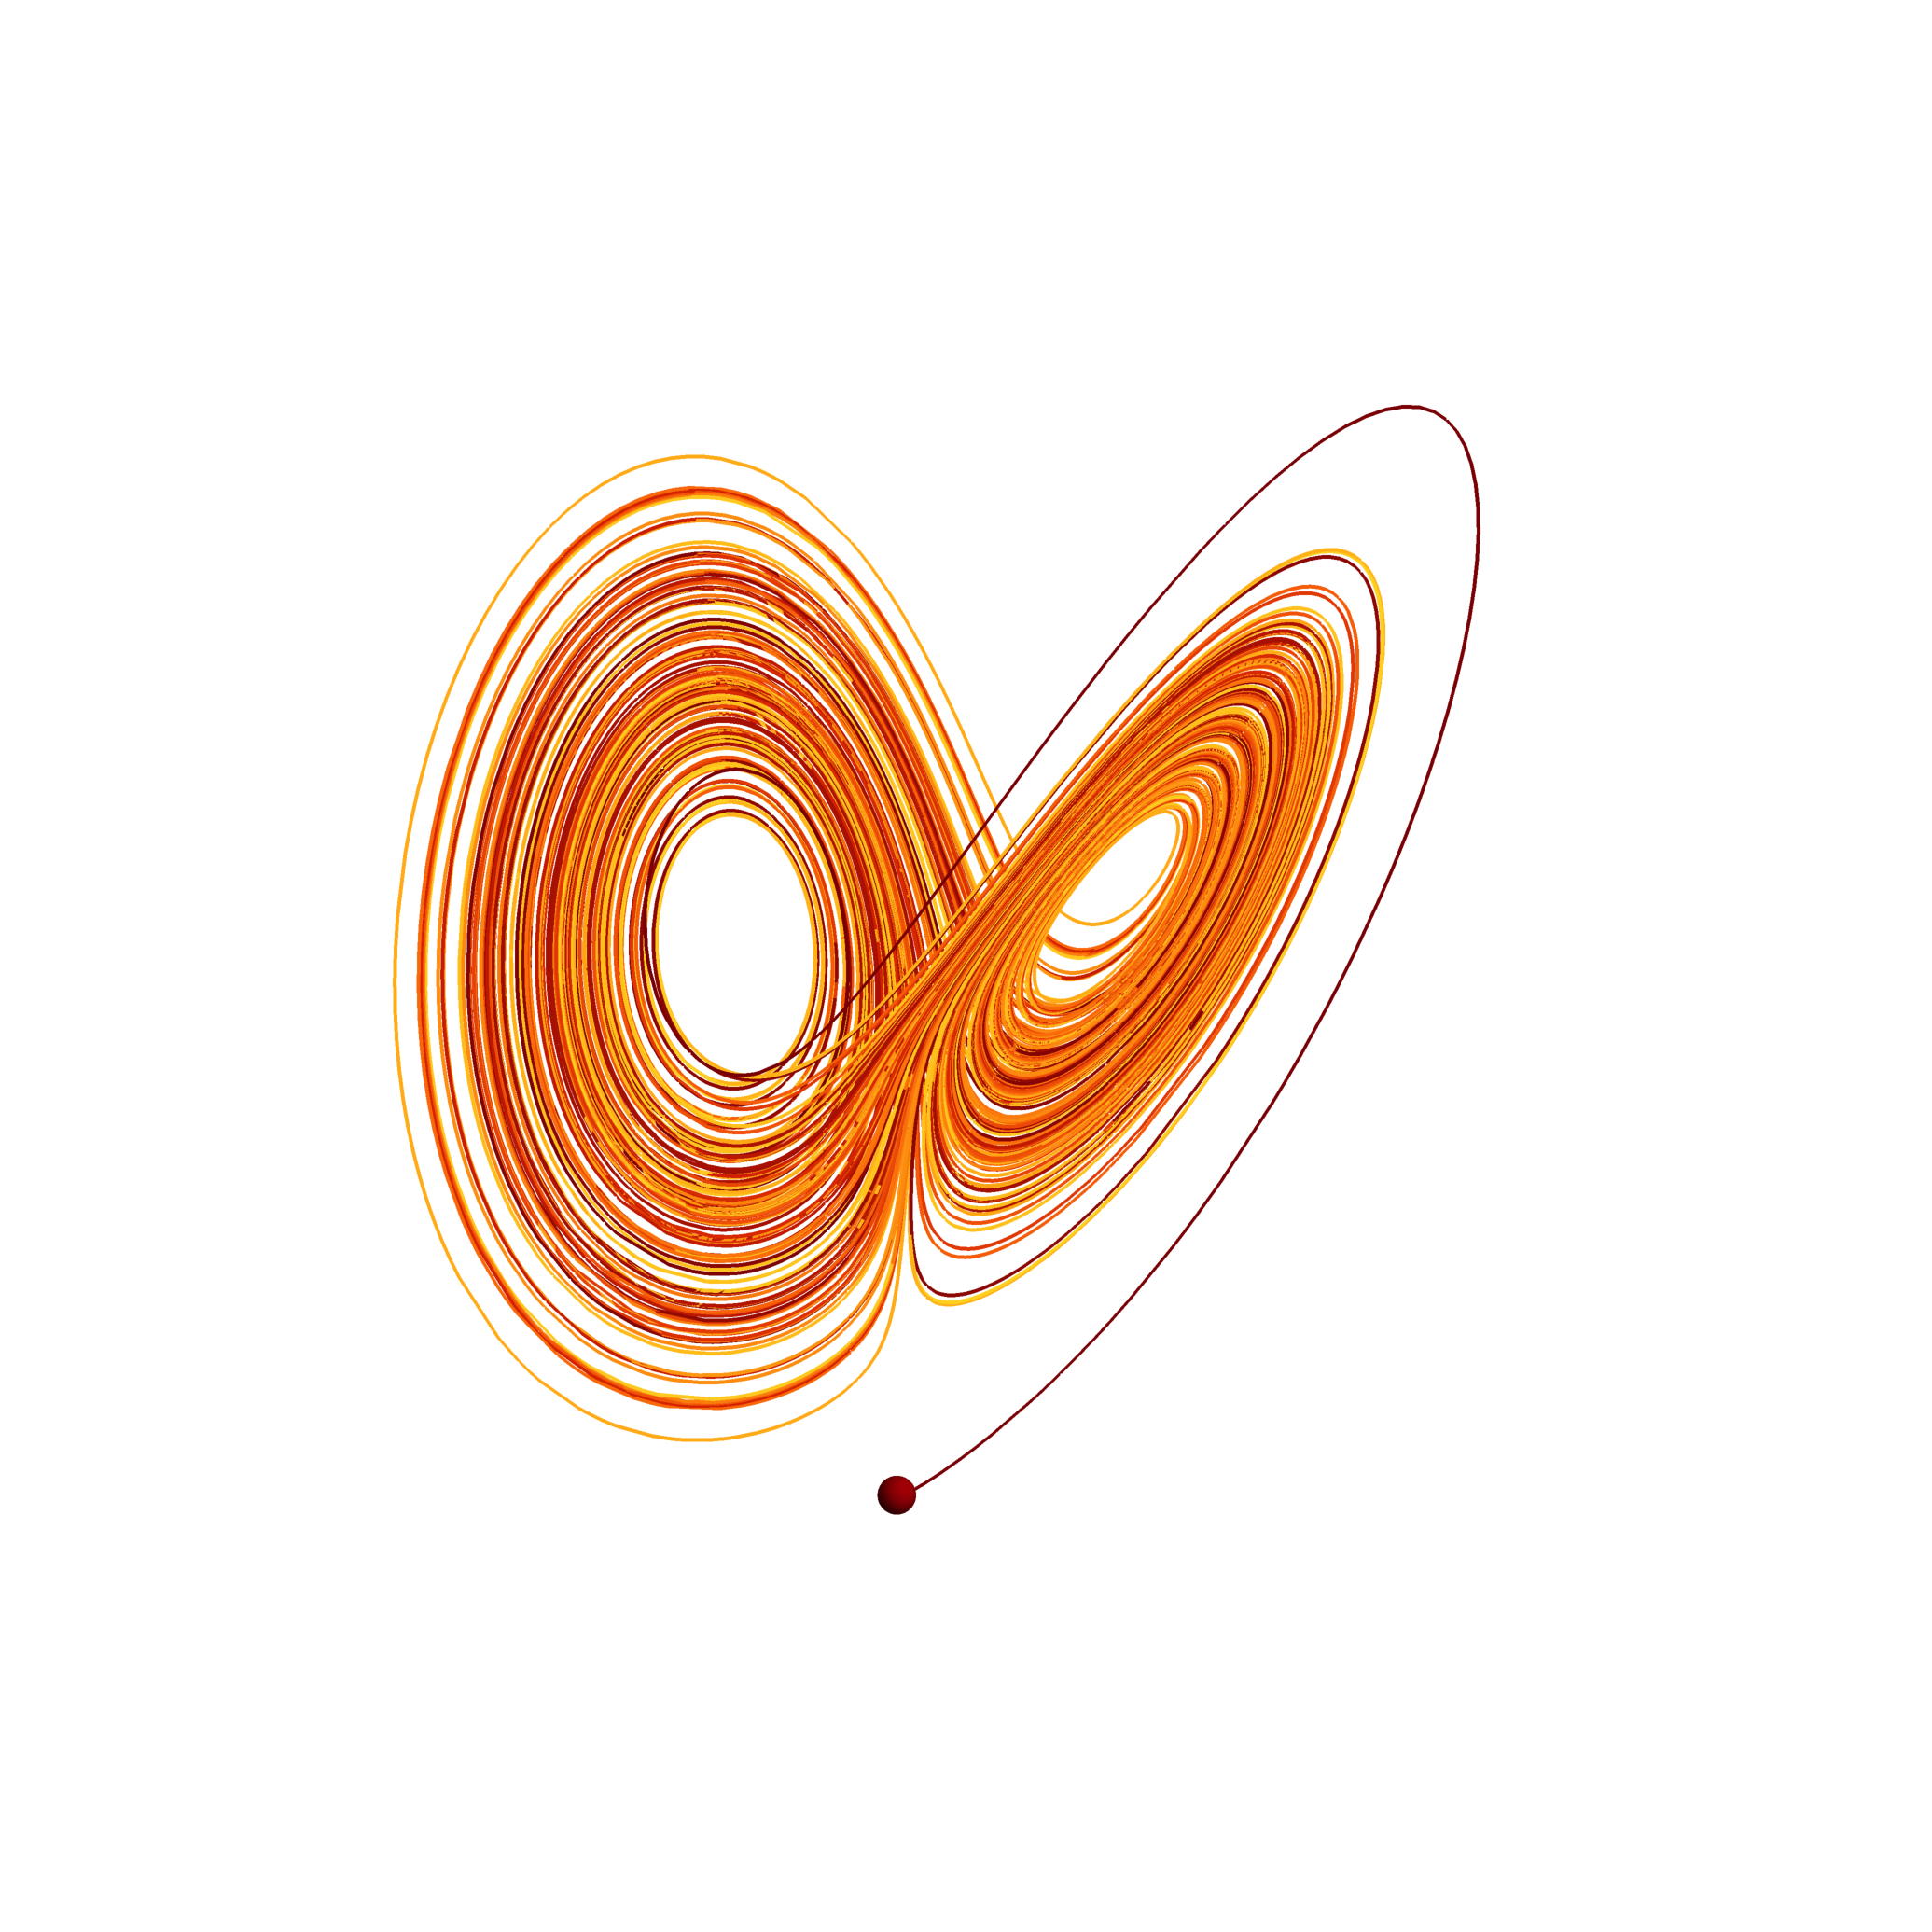
\includegraphics[width=0.55\textwidth]{include/mathematica_lorenz}
\end{figure}

%yea yea, I know, this is much larger than 1/3rd but it's the last image and the PDF exported from mathematica had a lot of whitespace making it look much smaller. 

This model is modeled in 3D, which shows more of the "Butterfly" principles that Lorenz described his discovery to be. All in all, Lorenz developed a mathematical principal that is still researched and modeled today. This model can help meteorologists, mathematicians and even members of the computer science community to help home their programming skills such as in this course. 


\begin{thebibliography}{9}

\bibitem{WolframA}
  Attractor.
  Wolfram Research, Inc.,
  \textit{Wolfram Mathworld},
  Weisstein, Eric W. "Attractor." From MathWorld--A Wolfram Web Resource.

\bibitem{WolframLA}
 Lorenz Attractor.
 Wolfram Research, Inc.,
 \textit{Wolfram Mathworld},
 Weisstein, Eric W. "Lorenz Attractor." From MathWorld--A Wolfram Web Resource.

 \bibitem{History}
 History.
 American Physics Society.
 Gleick, James. Chaos: Making a New Science, Viking Penguin, 1987.

 \bibitem{Mathematica}
 Wolfram.
 Wolfram Research, Inc.,
 \textit{Wolfram Reference}

 \end{thebibliography}




\end{document}





























